\documentclass[12pt]{article}
\usepackage[T1, T2A]{fontenc}
\usepackage[utf8]{inputenc}
\usepackage[russian]{babel}
\usepackage{hyperref}
\usepackage{graphicx}
\graphicspath{ {../Images/} }

\author{Григорий Матюхин}
\date{\today}
\title{Лабораторная работа \textnumero1.\\Установка и конфигурация операционной системы на виртуальную машину}

\begin{document}
  \maketitle
  \newpage
  \tableofcontents
  \newpage
  \section{Цель работы}
  Целью данной работы является приобретение практических навыков установки операционной системы на виртуальную машину, настройки минимально необходимых для дальнейшей работы сервисов.

  \section{Результат}
    Дождитесь загрузки графического окружения и откройте терминал. В окне терминала проанализируйте последовательность загрузки системы, выполнив команду \texttt{dmesg}. Получите следующую информацию.
    \begin{enumerate}
      \item Версия ядра Linux (Linux version).
        \\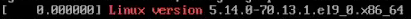
\includegraphics{1.png}\\
      \item Частота процессора (Detected Mhz processor).
        \\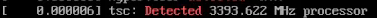
\includegraphics{2.png}\\
      \item Модель процессора (CPU0).
        \\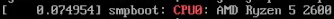
\includegraphics{3.png}\\
      \item Объем доступной оперативной памяти (Memory available).
        \\
\includegraphics{4.png}\\
      \item Тип обнаруженного гипервизора (Hypervisor detected).
        \\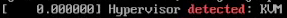
\includegraphics{5.png}\\
      \item Тип файловой системы корневого раздела.
        \\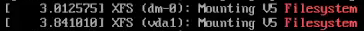
\includegraphics{6.png}\\
      \item Последовательность монтирования файловых систем.
        \\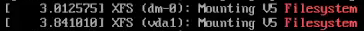
\includegraphics{6.png}\\
    \end{enumerate}
  \section{Контрольные вопросы}
    \begin{enumerate}
      \item Какую информацию содержит учётная запись пользователя?
        \\Учётная запись, как правило, содержит сведения, необходимые для опознания пользователя при подключении к системе, сведения для авторизации и учёта. Это идентификатор пользователя и его пароль.
      \item Укажите команды терминала и приведите примеры:
        \begin{enumerate}
          \item для получения справки по команде;
            \\\texttt{man}
            \\Пример:
            \\\texttt{man cat}, \texttt{man git}
          \item для перемещения по файловой системе;
            \\\texttt{cd}
            \\Пример:
            \\\texttt{cd} -- для перемещения в домашний каталог, \texttt{cd ..}, \texttt{cd Downloads}
          \item для просмотра содержимого каталога;
            \\\texttt{ls}
            \\Пример:
            \\\texttt{ls -l}, \texttt{ls Downloads}
          \item для определения объёма каталога;
            \\\texttt{du}
            \\Пример:
            \\\texttt{du -sh}, \texttt{du -sh \~}
          \item для создания / удаления каталогов / файлов;
            \\\texttt{touch file.txt} -- Создать файл
            \\\texttt{mkdir my\_dir} -- Создать каталог
            \\\texttt{rm file.txt} -- Удалить файл
            \\\texttt{rm -r my\_dir} -- Удалить каталог 
          \item для задания определённых прав на файл / каталог;
            \\\texttt{chmod}
            \\Пример:
            \\\texttt{chmod u+x executable\_file}
            \\\texttt{chmod g+w file\_to\_write\_to}
            \\\texttt{chmod o-r others\_cannot\_read}
          \item для просмотра истории команд.
            \\\texttt{history}
        \end{enumerate}
      \item Что такое файловая система? Приведите примеры с краткой характеристикой.
        \\Файловая система – это инструмент, позволяющий операционной системе и программам обращаться к нужным файлам и работать с ними.
        \\Ext2, Ext3, Ext4 или Extended Filesystem– стандартная файловая система, первоначально разработанная еще для Minix. Содержит максимальное количество функций и является наиболее стабильной в связи с редкими изменениями кодовой базы. Начиная с ext3 в системе используется функция журналирования. Сегодня версия ext4 присутствует во всех дистрибутивах Linux. 
        \\JFS или Journaled File System разработана в IBM в качестве альтернативы для файловых систем ext. Сейчас она используется там, где необходима высокая стабильность и минимальное потребление ресурсов (в первую очередь в многопроцессорных компьютерах). В журнале хранятся только метаданные, что позволяет восстанавливать старые версии файлов после сбоев.
        \\ReiserFS такжеразработана в качестве альтернативы ext3, поддерживает только Linux. Динамический размер блока позволяет упаковывать несколько небольших файлов в один блок, что предотвращает фрагментацию и улучшает работу с небольшими файлами. Недостатком является риск потери данных при отключении энергии. 
        \\XFS рассчитана на файлы большого размера, поддерживает диски до 2 терабайт. Преимуществом системы является высокая скорость работы с большими файлами, отложенное выделение места, увеличение разделов на лету, незначительный размер служебной информации. К недостаткам относится невозможность уменьшения размера, сложность восстановления данных и риск потери файлов при аварийном отключении питания.
        \\Btrfs или B-Tree File System легко администрируется, обладает высокой отказоустойчивостью и производительностью. Используется как файловая система по умолчанию в OpenSUSE и SUSE Linux.
      \item Как посмотреть, какие файловые системы подмонтированы в ОС?
        \\Используя команду \texttt{findmnt}
      \item Как удалить зависший процесс?
        \\ Используя команду \texttt{kill}
    \end{enumerate}
  \section{Вывод}
    В ходе выполнения данной работы я приобрел практические навыков установки операционной системы на виртуальную машину, настройки минимально необходимых для дальнейшей работы сервисов. 
\end{document}
